% - - - - - - - - - - - - - - - - - - - - - - - - - - - - 
\subsection{PROC-03 Agregar medicamento del proveedor}

\begin{figure}[htbp]
	\begin{center}
		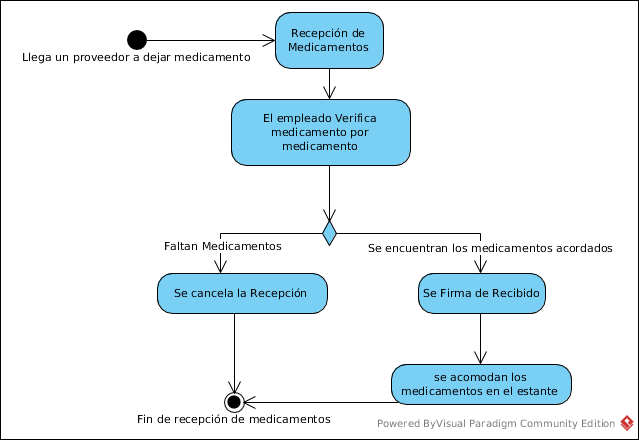
\includegraphics[width=.7\textwidth]{images/as-toprocAgreMedic}
		\caption{PROC-03 Agregar medicamento del proveedor}
		\label{fig:proceso1}
	\end{center}
\end{figure}

\begin{description}
	\item[Descripción:] Son Acciones realizadas por el empleado de planta en la farmacia, sucede cuando un proveedor trae una entrega, el empleado tiene que verificar que los medicamentos son los que se pidieron y procede a Firmar,pagar y acomodar los medicamentos en su  estante
	\item[Entradas:] \cdtEmpty
        \begin{itemize}
			\item Medicamentos.
			\item Nota de recibido.
        \end{itemize}
	\item[Salidas:] \cdtEmpty
        \begin{itemize}
			\item Dinero
			\item Medicamentos caducados
        \end{itemize}	
    \item[Áreas de oportunidad:] Con el sistema le sera más fácil controlar 
    El ingreso de medicamentos por un proveedor, si bien se tendrá que hacer un proceso más largo, este ayudara al empleado a entregar cuentas al supervisor de la sucursal.
     \end{description}
